\chapter{Properties of the Euler-Voigt Equations}

\section{Finite Time Blow-up Criterion}\label{sec:blowup:criterion}

In order to begin our search for finite-time singularity formation, we must first describe the {\color{red}criteria used to detect singularity formation in Euler flows. In \cite{larios_higher-order_2010} a new criterion for identifying singularity formation in Euler flows was developed which utilizes the Euler-Voigt equations. This criterion began relies on} the convergence of the solutions of (\ref{eq:Euler:Voigt}) to the solutions of (\ref{eq:Euler}) as $\alpha\rightarrow 0$. 
\begin{thm}[\cite{larios_higher-order_2010}]\label{thm:Theorem:1.2}
Given initial data $\be,\bea \in H^s(\TT^3)$ for some $s\geq 3$, let $\u,\ua \in C([0,T],H^s(\Omega))\cap C^1([0,T],H^{s-1}(\Omega))$ be the corresponding solutions to (\ref{eq:Euler}) and (\ref{eq:Euler:Voigt}), respectively, where $0<T<T_{\text{max}}$ and $T_{\text{max}}$ is the maximal time for which a solution to (\ref{eq:Euler}) exists and is unique. For all $t\in[0,T]$, we have 
\begin{equation}
\begin{aligned}
\|\u(t)-\ua(t)\|_{L^2}^2 + \alpha^2\|\bn(\u(t)-\ua(t))\|_{L^2}^2 \leq \\ \left( \|\be-\bea \|_{L^2}^2 + \alpha^2\|\bn(\be - \bea)\|_{L^2}^2 \right)e^{Ct} + C\alpha^2(e^{Ct}-1).
\end{aligned}
\end{equation}
\end{thm}
\noindent {\color{red}Here we denote $H^s$ as the Sobolev space over the domain $\Omega$, and $C^k$ as the space of $k$-times differentiable functions on $\Omega$}. Based on this theorem we know that if
\begin{equation}\label{eq:eta:0:condition}
\|\be-\bea\|_{L^2}^2+\alpha^2\|\bn(\be-\bea)\|_{L^2}^2 \rightarrow 0, \quad \text{as } \alpha\rightarrow 0,
\end{equation}
then for all $t\in [0,T]$,
\begin{equation}
\|\u(t)-\ua(t)\|_{L^2}^2 + \alpha^2\|\bn(\u(t)-\ua(t))\|_{L^2}^2 \rightarrow 0.
\end{equation}
{\color{red}Therefore solutions of the Euler-Voigt system (\ref{eq:Euler:Voigt}) converge to the corresponding Euler (\ref{eq:Euler}) flows in $H^1$ uniformly in time as $\alpha\rightarrow 0$. Using this result, the following theorem was proved in \cite{larios_computational_2018}}.

\begin{thm}\label{thm:Theorem:1.1}
Let $\bea\in H^s$, $s\geq 3$, with $\bn \cdot \ea = 0$ and let $\ua$ be the corresponding unique solution of (\ref{eq:Euler:Voigt}). Suppose that there exists a time $T^*>0$ such that
\begin{equation}
\limsup_{\alpha \rightarrow 0^+} \left( \alpha \sup_{t\in[0,T^*]} \|\bn \ua(t)\|_{L^2}\right) > 0.
\end{equation}
Then {\color{red}the corresponding solution of the Euler} equations (\ref{eq:Euler}) with the initial condition $\be_\alpha$ must develop a singularity within the interval $[0,T^*]$.
\end{thm}
\noindent We note that this theorem relies on {\color{red}the solutions of} (\ref{eq:Euler}) and (\ref{eq:Euler:Voigt}) starting from the same initial condition, i.e. $\be = \bea$. This necessarily satisfies (\ref{eq:eta:0:condition}) as $\alpha\rightarrow 0$. However, in order to use this {\color{red} result in our study, we need to generalize Theorem \ref{thm:Theorem:1.1} for the case} (\ref{eq:eta:0:condition}) where $\be \neq \bea$. Therefore, we modify Theorem 5.2 from \cite{larios_higher-order_2010} as follows. \begin{thm}[{\color{red}X. Zhao, private communication}]\label{thm:Theorem:1.3}
Given initial data $\be,\bea \in H^s(\TT^3)$ for some $s\geq 3$ satisfying
\begin{equation}
\|\be-\bea\|_{L^2}^2+\alpha^2\|\bn(\be-\bea)\|_{L^2}^2 \rightarrow 0, \quad \text{as } \alpha\rightarrow 0,
\end{equation} 
let $\u,\ua \in C([0,T],H^s(\TT^3))\cap C^1([0,T],H^{s-1}(\TT^3))$ be the corresponding solutions to (\ref{eq:Euler}) and (\ref{eq:Euler:Voigt}), respectively. If there exists a finite time $T^*>0$ such that the solutions $\ua$ satisfy
\begin{equation}
\limsup_{\alpha \rightarrow 0} \left( \alpha^2 \sup_{t\in[0,T^*]} \|\bn \ua(t)\|_{L^2}^2\right) > 0,
\end{equation}
then $\u$ develops a singularity in the interval $[0,T^*]$.
\end{thm}

\begin{proof}
Suppose that the solution $\u$ of the Euler equations (\ref{eq:Euler}) with the initial condition $\be$ is regular on $[0,T^*]$. Since the Euler-Voigt equations are globally well-posed, we have, {\color{red}cf. (\ref{eq:alpha:Energy})}
\begin{equation}
\|\ua(t)\|_{L^2}^2 + \alpha^2\|\bn\ua(t)\|_{L^2}^2  = \|\bea\|_{L^2}^2+\alpha^2\|\bn\bea\|_{L^2}^2,
\end{equation}
thus
\begin{equation}
\alpha^2\|\bn\ua(t)\|_{L^2}^2  = \|\bea\|_{L^2}^2+\alpha^2\|\bn\bea\|_{L^2}^2 - \|\ua(t)\|_{L^2}^2.
\end{equation}
Taking the supremum over $t\in[0,T^*]$ of the above equation, we obtain that
\begin{equation}
\sup_{t\in[0,T^*]}\alpha^2\|\bn\ua(t)\|_{L^2}^2  = \|\bea\|_{L^2}^2+\alpha^2\|\bn(\bea)\|_{L^2}^2 - \inf_{t\in[0,T^*]} \|\ua(t)\|_{L^2}^2.
\end{equation}
Taking the limsup as $\alpha\rightarrow 0$, we obtain 
\begin{equation}
\limsup_{\alpha\rightarrow 0}\left(\sup_{t\in[0,T^*]}\alpha^2\|\bn\ua(t)\|_{L^2}^2\right)  = \limsup_{\alpha\rightarrow 0}\left(\|\bea\|_{L^2}^2+\alpha^2\|\bn(\bea)\|_{L^2}^2 - \inf_{t\in[0,T^*]} \|\ua(t)\|_{L^2}^2\right).
\end{equation}
We now make use of Theorem \ref{thm:Theorem:1.2}, which demonstrates that the convergence of the solutions of the Euler-Voigt equations (\ref{eq:Euler:Voigt}) to the solution of the Euler equations (\ref{eq:Euler}) is uniform on $[0,T^*]$. Therefore we can reduce the above equation to
\begin{equation}\label{eq:second:equality}
\limsup_{\alpha\rightarrow 0}\left(\sup_{t\in[0,T^*]}\alpha^2\|\bn\ua(t)\|_{L^2}^2\right)  = \|\be\|_{L^2}^2 - \|\u(t)\|_{L^2}^2.
\end{equation}
Since the energy of regular solutions of the Euler equations is conserved, we have
\begin{equation}
\limsup_{\alpha\rightarrow 0}\left(\sup_{t\in[0,T^*]}\alpha^2\|\bn\ua(t)\|_{L^2}^2\right)  = 0,
\end{equation}
which contradicts the hypothesis in the theorem that the above expression is positive. Equality (\ref{eq:second:equality}) holds because
\begin{subequations}
\begin{align*}
\limsup_{\alpha\rightarrow 0}\left| \inf_{t\in[0,T^*]} \|\ua(t)\|_{L^2} - \|\be\|_{L^2} \right| &\leq \limsup_{\alpha\rightarrow 0}\|\ua(t_\alpha) - \be\|_{L^2}^2 \\
&\leq \limsup_{\alpha\rightarrow 0}\|\ua(t_\alpha) - \u(t_\alpha)\|_{L^2}^2 + \|\u(t_\alpha) - \be\|_{L^2}^2 \\
&= 0,
\end{align*}
\end{subequations}
{\color{red}where the reverse triangle and triangle inequalities were used and $t_\alpha$ is the time at which
\begin{equation}
\inf_{t\in[0,T^*]} \|\ua(t)\|_{L^2} = \|\ua(t_\alpha)\|_{L^2}
\end{equation}
}

\end{proof}


\section{Initial Conditions}\label{sec:initial:conditions}

We have established {\color{red}Theorem \ref{thm:Theorem:1.3}} which we will use identify singularity formation in Euler flows from smooth initial conditions. In order to formulate our optimization problem we must now describe the function space we perform our search in. The theorems (\ref{thm:Theorem:1.2}), (\ref{thm:Theorem:1.1}), and (\ref{thm:Theorem:1.3}) presented in Section (\ref{sec:blowup:criterion}) require initial conditions $\be,\bea \in H^s(\TT^3)$ for some $s\geq 3$. However, the pseudo-spectral methods used in this study {\color{red} to numerical solve system (\ref{eq:Euler:Voigt}) require the functions to be analytic in order to have exponential convergence \cite{canuto_spectral_2006}. For the Navier-Stokes equations (\ref{eq:Navier:Stokes}), the viscous term acts to instantaneously regularize the solution in space. Therefore, if the initial condition has only Sobolev regularity, the resulting flow becomes real-analytic (with Gevrey regularity defined below) at $t=0^+$. This regularity allows the solution to achieve exponential convergence.}
\\~\\
For the Euler equations (\ref{eq:Euler}) there is no viscosity and so the solution simply stays at the same level of smoothness as the initial condition{\color{red}, unless blow-up occurs}. For Euler-Voigt the regularization term keeps the solution globally well-posed but does not improve the regularity \cite{larios_higher-order_2010}. Therefore, we must have analytic initial conditions to make use of the pseudo-spectral methods. For {\color{red}all the models considered here, a requirement is that the fluid is divergence free at all times, including the initial conditions. Finally, on a periodic domain the quantity $\int_\Omega \bea \,d\x$ is an invariant of motion for solutions of the Euler-Voigt equations.} Due to this, we assume without loss of generality that the initial conditions have a mean of zero. In order to identify initial conditions that satisfy these criteria, we first consider analytic initial conditions that belong to the Gevrey class
\begin{equation}\label{eq:Gevrey:Class}
G^\sigma := \lb \v\in H^s(\TT^3) : \|\v\|_{G^\sigma} = \la \v,\v\ra_{G^\sigma}^{1/2}<\infty \rb, \quad s\geq 3, \quad \sigma > 0,
\end{equation}
with the norm defined as
\begin{subequations}\label{eq:Gevrey:Inner:Product}
\begin{align}
\forall \v,\u \in G^\sigma, \quad \la \v,\u \ra_{G^\sigma} :=& \sum_{\j\in \ZZ^3} (1+|2\pi \j|^2)^se^{4\pi\sigma|\j|}\widehat{\v}_{\j}\cdot \overline{\widehat{\u}}_{\j} \\
=& \int_{\TT^3}(1+|D|^2)^se^{2\sigma |D|}\v\cdot \u \, d\x,
\end{align}
\end{subequations}
where hat denotes the Fourier coefficient{\color{red}
\begin{equation}
\widehat{v}_k = \frac{1}{N} \sum_{j=1}^N e^{-ikx_j}v_j,
\end{equation}}
\noindent overbar denotes complex conjugation, and the operators $|D|$ and $e^{\sigma|D|}$ are defined via
\begin{equation}\label{eq:D}
\left[ \widehat{|D|\boldsymbol v} \right]_{\boldsymbol j} := 2\pi|\boldsymbol j|\boldsymbol{\hat{v}_j}, \qquad \left[ \widehat{e^{\sigma |D|}\boldsymbol v} \right]_{\boldsymbol j} := e^{2\pi|\boldsymbol j|}\boldsymbol{\hat{v}_j}.
\end{equation}
The parameter $\sigma$ determines the {\color{red}relative 'size'} of the Gevrey space
\begin{equation}\label{eq:Gevrey:size}
G^{\sigma_2} \subset G^{\sigma_1} \subset G^0 = H^s, \quad 0 < \sigma_1 < \sigma_2,
\end{equation}
which is proved in Appendix \ref{app:Gevrey:size}. The value of $\sigma$ is chosen in Section \ref{sec:sigma}. In order to satisfy the divergence free condition, we introduce the following subspace in which optimal initial conditions will be sought
\begin{equation}\label{eq:subspace:v}
V := \{\boldsymbol v \in G^\sigma : \boldsymbol \nabla \cdot \boldsymbol v = 0, \quad \int_{\mathbb{T}^3}\boldsymbol v\, d\x = 0\}.
\end{equation}

\section{Scaling Symmetries of Euler and Euler-Voigt Systems}

{\color{red}Both (\ref{eq:Euler}) and (\ref{eq:Euler:Voigt}) possess a scaling property. Given a solution $\u_{(\alpha)}$ we can construct a new solution
\begin{equation}\label{eq:time:scaling}
\tilde{\u}_{(\alpha)}(\y,\tau) = \frac{1}{\gamma}\u_{(\alpha)}(\beta\x,\lambda t), \qquad \y = \beta \x, \qquad \tau = \lambda t
\end{equation}
which is a valid solution of the Euler-Voigt equations (\ref{eq:Euler:Voigt}) when $\lambda,\gamma,\beta >0$ satisfy $\beta/\lambda\gamma = 1$, which is proven in Appendix \ref{app:time:scale:euler} and \ref{app:time:scale:euler:voigt}. Our goal is to find an time interval $[0,T]$ that is sufficiently large so that it is outside the interval of local existence established by Kato's theorem \cite{beale_remarks_1984} and so allows for the potential of singularity formation in Euler.} Due to this scaling property of the Euler-Voigt equations (\ref{eq:time:scaling}), the blow-up time of the solution will depend on the 'size' of our solution ($\gamma$) and the spatial scale ($\beta$). Our domain size will not change, and so in order to keep consistent time scale we must fix $\gamma$ between all initial conditions. {\color{red}To accomplish this, we restrict our discussion to initial conditions with a fixed $\hdo$ seminorm which belong to a closed manifold $\M_C\subset V$ defined as
\begin{equation}\label{eq:manifold}
\M_C = \{\v \in V : \|\v\|_{\hdo} = C \},
\end{equation}
where $C>0$ is a constant. We create the manifold by fixing the $\hdo$ seminorm because of the form of our objective functional used in the optimization search, which will be described in Chapter \ref{chp:optimization:problem}.} The question we must answer now is what value of $C$ we use. To determine this we look to our first initial condition, the 3D Taylor Green Vortex (TGV). The TGV in the domain $\Omega=[0,L]^3$ has the form
\begin{equation}\label{eq:TGV}
\be_{TGV}(x) = \begin{bmatrix}
V_0\sin(2\pi x/L)\cos(2\pi y/L)\cos(2\pi z/L) \\
-V_0\cos(2\pi x/L)\sin(2\pi y/L)\cos(2\pi z/L) \\
0
\end{bmatrix},
\end{equation}
for some $V_0\neq 0$. The $\hdo$-seminorm of (\ref{eq:TGV}) is
\begin{equation}
\|\be_{TGV}\|_{\hdo} = \sqrt{3L}\pi V_0,
\end{equation}
which is proven in Appendix (\ref{app:tg:seminorm:general}). In addition, the BKM criterion (\ref{eq:beale:kato:majda}) uses the quantity $\|\bds\omega\|_{L^\infty}$ to determine singularity formation. For the TGV
\begin{equation}
\|\bds\omega\|_{L^\infty} = \|\nabla\times\be_{TGV}\|_{L^\infty} = 4\pi V_0/L,
\end{equation}
which is proven in Appendix (\ref{app:tg:vorticity:general}). {In \cite{bustamante_interplay_2012}, the authors provided numerical evidence that blow-up of (\ref{eq:Euler}) may occur around $T^* \approx 4$ for initial condition (\ref{eq:TGV}) with parameters $L=1$ and $V_0=1$. This result provides the baseline for our study and so we must match this time window so that singularity formation identified by (\ref{thm:Theorem:1.3}), if it happens, occurs at approximately the same time as in \cite{bustamante_interplay_2012}. Therefore, we set $\lambda = 1$. Our Euler-Voigt system is defined on the domain $\Omega=[0,1]^3$ }and so we set $\beta = 1/2\pi$. Therefore, from (\ref{eq:time:scaling}) we set $\gamma = 1/2\pi$. The model we are aiming to match uses $V_0=1$ and so to match the time window we use $V_0 = 1/2\pi$.
\\~\\ 
{\color{red}These considerations give $\|\eta_{TGV}\|_{\hdo} = \sqrt{3}/2$ and $\|\nabla\times\eta_{TGV}\|_{L^\infty} = 2$ for the initial condition (\ref{eq:TGV})}. Therefore, we can restrict our discussion of the TGV to initial conditions with $\hdo$ seminorm which belong to a closed {\color{red}manifold \ref{eq:manifold} with $C=\sqrt{3}/2$}. In order to select initial conditions within this manifold, we will first select initial conditions $\be\in V$ and then apply a retraction function to ensure it has $\|\cdot\|_{\hdo} = \sqrt{3}/2$. {\color{red}To verify that this selection for the initial $\hdo$ seminorm is correct we compare this scaling to the results shown in Figure 1b of  \cite{bustamante_interplay_2012}. This figure shows the evolution of the $L^\infty$ norm of the vorticity over time. }

\begin{figure}[h!]\label{fig:scaled:vorticity}
  \centering
  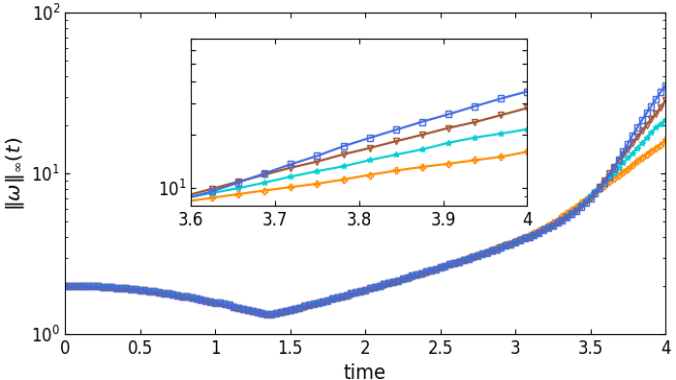
\includegraphics[width=.8\linewidth]{figures/Figure_1.png}
  \caption{Maximum of vorticity $\|\omega(\cdot,t)\|_\infty$. Results from runs performed at different resolutions are displayed together: $128^3$ (orange plus), $256^3$ (cyan star), $512^3$ (brown triangles), $1024^3$ (blue squares).}
\end{figure}

{\color{red}\noindent We present our reproduction in Figure \ref{fig:scaled:vorticity}. Figure \ref{fig:scaled:vorticity} shows that the evolution of the vorticity at each resolution in our scaled model matches exactly to the corresponding resolutions of Figure 1b in \cite{bustamante_interplay_2012}. Therefore, our selection for the manifold $\M_C$ is correct.}